% !TeX spellcheck = fr_FR
\documentclass[a4paper,11pt,oneside,roman]{article}
    \usepackage[utf8]{inputenc}
    \usepackage[T1]{fontenc}
    \usepackage[top=2cm, left=2cm, right=2cm, bottom=2cm]{geometry}
    \usepackage[francais]{babel}
    \usepackage[hidelinks=true]{hyperref}
    \usepackage{listings}
    \usepackage{color}
    \usepackage{amsmath}
    \usepackage{graphicx}
    \usepackage{amssymb}
    \usepackage{natbib}
    \usepackage{float}
    \usepackage{hyperref}
    \usepackage{advdate}
    \usepackage{caption}
    \usepackage{subcaption}
    
    \floatplacement{figure}{H}
    
    \definecolor{dkgreen}{rgb}{0,0.6,0}
    \definecolor{gray}{rgb}{0.5,0.5,0.5}
    \definecolor{mauve}{rgb}{0.58,0,0.82}
    
    \linespread{1.3} %space between lines
    \setlength{\parskip}{1em}  %space between paragraphs
    
    \begin{document}
    
    \begin{titlepage}
    
        \newcommand{\HRule}{\rule{\linewidth}{0.5mm}} % Defines a new command for the horizontal lines, change thickness here
        
        \center % Center everything on the page
         
        %----------------------------------------------------------------------------------------
        %	HEADING SECTIONS
        %----------------------------------------------------------------------------------------
        
        \textsc{\LARGE Université de Technologie de Compiègne}\\[0.5cm] % Name of your university/college
        \textsc{\Large Génie informatique}\\[1.5cm] % Name of your university/college
        
        %----------------------------------------------------------------------------------------
        %	TITLE SECTION
        %----------------------------------------------------------------------------------------
        
        \HRule \\[0.4cm]
        { \huge \bfseries Rapport du projet de SY09}\\[0.4cm] % Title of your document
        \HRule \\[1.5cm]
         
        %----------------------------------------------------------------------------------------
        %	AUTHOR SECTION
        %----------------------------------------------------------------------------------------
        
        % If you don't want a supervisor, uncomment the two lines below and remove the section above
        \Large \emph{Authors:}\\
        Antoine \textsc{Collas} et Julien \textsc{Crauser}\\[3cm] % Your name
        
        %----------------------------------------------------------------------------------------
        %	DATE SECTION
        %----------------------------------------------------------------------------------------
        
        {\large \AdvanceDate[-4]\today}\\[4cm] % Date, change the \today to a set date if you want to be precise
        
        %----------------------------------------------------------------------------------------
        %	LOGO SECTION
        %----------------------------------------------------------------------------------------
        
        
\includegraphics[width=0.5\textwidth]{imgs/logo_UTC_SU.jpg}\\[1cm] % Include a department/university logo - this will require the graphicx package
        
        %----------------------------------------------------------------------------------------
    
        \vfill % Fill the rest of the page with whitespace
        
    \end{titlepage}
    
    % \tableofcontents
    
    \pagebreak
        
    \section{Cuisine}
    \subsection*{Question 1}
    Le jeu de données présent dans le fichier recettes-pays.data contient 51 variables pour 26 individus.
    Nous pouvons donc noter que nous disposons de plus de variables que d'individus.
    Parmi ces 51 variables, une seule est qualitative (les origines des recettes) et 50 sont quantitaves.
    Ces dernières prennent leurs valeurs entre $0$ et $1$ ($0$ et $0.82$ pour être plus précis).
    Dans ce jeux de données les recettes ont été agrégées par origine, il y a donc 26 origines (une par ligne de notre tableau individus-variables).
    De plus, le jeu de données ne présente aucunes valeurs manquantes.
    Cependant certaines origines sont à remarquer.
    En effet, il y a par exemple une distinction entre l'Afrique et le Maroc ou encore entre l'Asie et Chine, Japon, Vietnam, Thailande.
    De plus, les origines semblent être regroupées par région géographique mais des origines comme \"juive\",\"cadiens\", sont présentes.

    \subsection*{Question 2}
    Nous réalisons une ACP sur le jeu de données. Nous obtenons 26 axes principaux: autant que d'individus.
    En effet, comme il y a moins d'individus que de variables, il est suffisant de prendre 26 axes pour représenter tous les individus.

    Nous obtenons les pourcentages d'inertie expliquée visibles sur la figure \ref{fig_acp}. 
    Les 3 premiers axes représentent $72\%$ de la variance du nuage de points.


    \begin{figure}
        \centering
        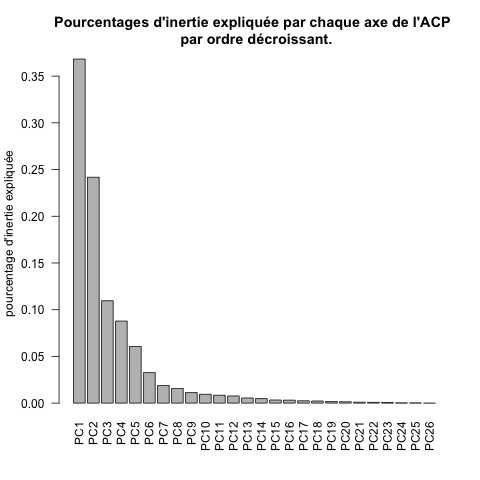
\includegraphics[width=0.5\textwidth]{imgs/acp.png}
        \caption{Pourcentages d'inertie expliquée}
        \label{fig_acp}
    \end{figure}

    Comme les 3 premiers axes factoriels représentent $72\%$ de la variance totale, nous analysons le nuage de points seulement avec les 3 premiers plans factoriels.
    Nous obtenons les plans factoriels des figures \ref{fig_acp_plan_1_2}, \ref{fig_acp_plan_1_3} et \ref{fig_acp_plan_2_3}. Nous avons associé à chaque plan son cercle des corrélations.
    
    \begin{figure}
        \centering
        \begin{subfigure}{.5\textwidth}
          \centering
          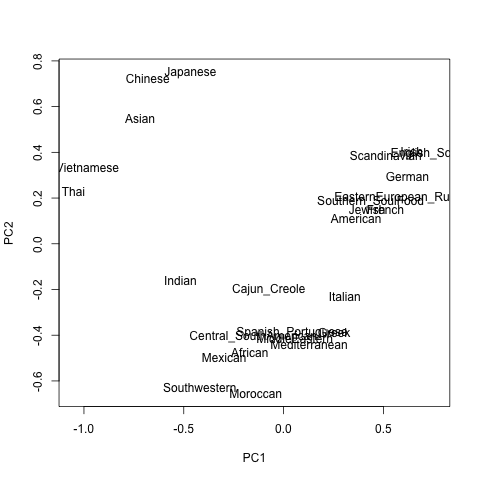
\includegraphics[width=.8\linewidth]{imgs/acp_plan_1_2.png}
          \caption{Plan 1,2}
          \label{fig:sub1}
        \end{subfigure}%
        \begin{subfigure}{.5\textwidth}
          \centering
          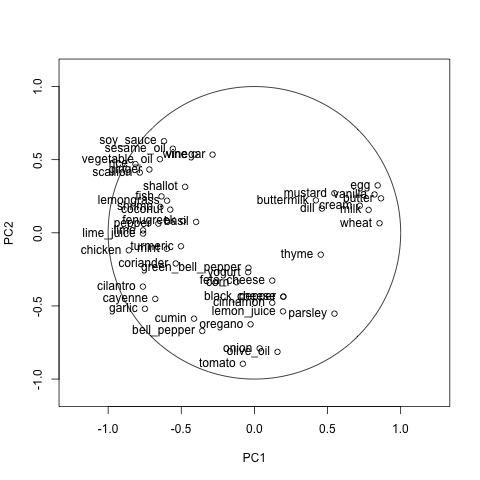
\includegraphics[width=.8\linewidth]{imgs/cercle_plan_1_2.png}
          \caption{Cercle des corrélations}
          \label{fig:sub2}
        \end{subfigure}
        \caption{Plan factoriel 1,2 avec son cercle associé}
        \label{fig_acp_plan_1_2}
    \end{figure}

    \begin{figure}
        \centering
        \begin{subfigure}{.5\textwidth}
          \centering
          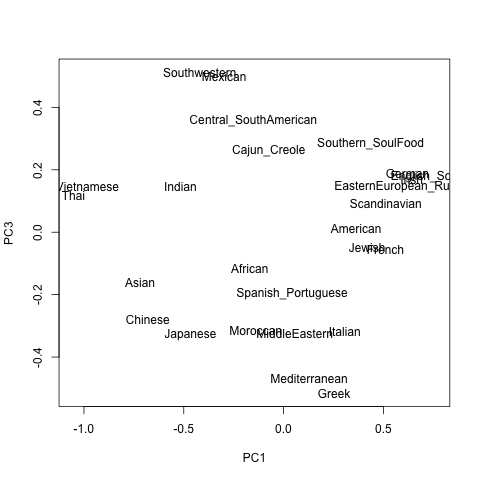
\includegraphics[width=.8\linewidth]{imgs/acp_plan_1_3.png}
          \caption{Plan 1,3}
          \label{fig:sub1}
        \end{subfigure}%
        \begin{subfigure}{.5\textwidth}
          \centering
          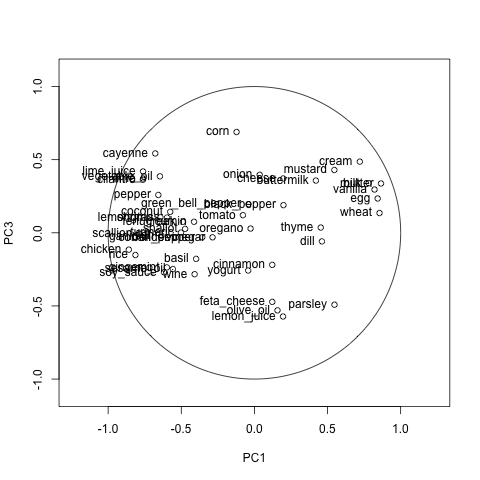
\includegraphics[width=.8\linewidth]{imgs/cercle_plan_1_3.png}
          \caption{Cercle des corrélations}
          \label{fig:sub2}
        \end{subfigure}
        \caption{Plan factoriel 1,3 avec son cercle associé}
        \label{fig_acp_plan_1_2}
    \end{figure}


    \begin{figure}
        \centering
        \begin{subfigure}{.5\textwidth}
          \centering
          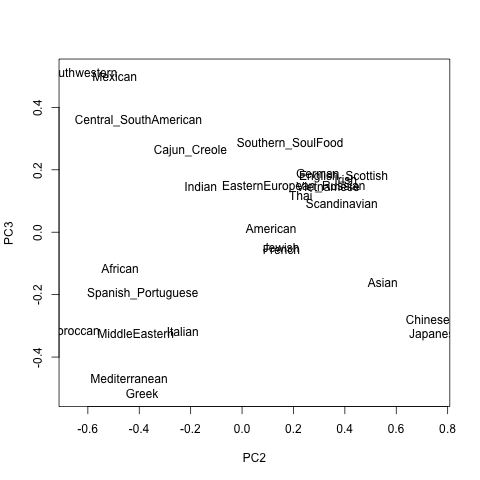
\includegraphics[width=.8\linewidth]{imgs/acp_plan_2_3.png}
          \caption{Plan 2,3}
          \label{fig:sub1}
        \end{subfigure}%
        \begin{subfigure}{.5\textwidth}
          \centering
          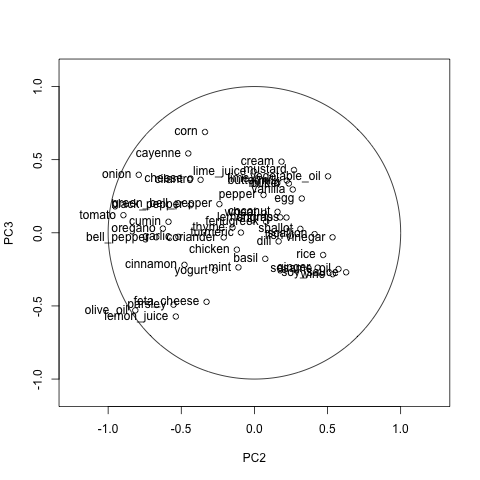
\includegraphics[width=.8\linewidth]{imgs/cercle_plan_2_3.png}
          \caption{Cercle des corrélations}
          \label{fig:sub2}
        \end{subfigure}
        \caption{Plan factoriel 2,3 avec son cercle associé}
        \label{fig_acp_plan_2_3}
    \end{figure}

    Dans le premier plan factoriel, nous observons que plusieurs groupes se forment.
    Les pays asiatiques se distinguent avec des ingrédients comme l'huile de sésame, l'huile de soja, le poisson, les échalottes...
    Un deuxième groupe se distingue: la cuisine occidentale avec des ingrédients comme le blé, les oeufs et le lait.
    Aussi, les pays consommant de la tomate et de l'huile d'olive sont exposés dans ce premier plan: Maroc, Mexique et Afrique.

    Dans le deuxième plan factoriel, la Grèce et la méditerranée sont liées par leur consommation de féta, d'huile d'olive et de jus de citron. 
    Ce plan permet aussi de voir la formation de deux sous groupes parmi les pays asiatiques.
    Le Vietnam et la Thaïlande consomment du poulet et du piment, ce qui est moins le cas de la Chine et du Japon.

    Enfin le troisième plan factoriel met en évidence des pays consommant du maïs comme le Mexique.

    \subsection*{Question 3}
    Nous obtenons le dendrogramme de la figure \ref{fig_CAH_dendrogramme}.
    
    \begin{figure}
        \centering
        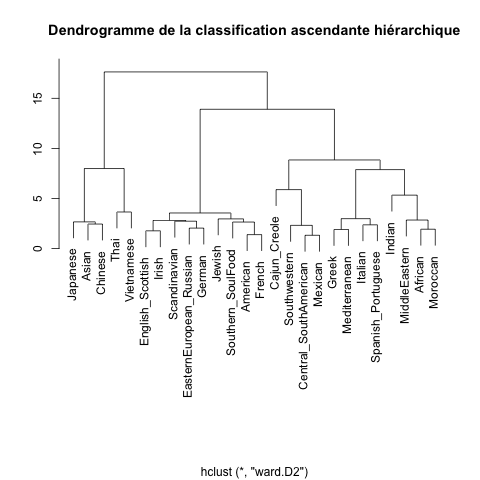
\includegraphics[width=0.5\textwidth]{imgs/CAH_dendrogramme.png}
        \caption{Dendrogramme de la classification ascendante hiérarchique}
        \label{fig_CAH_dendrogramme}
    \end{figure}

    Ce dendrogramme confirme plusieurs observations que nous avions déjà indiquées dans la deuxième question:
    \begin{itemize}
        \item les cuisines des pays asiatiques sont ensemble avec deux sous groupes: Japon-Chine, Thailande-Vietnam.
        \item les recettes de deux pays occidentaux, les Etats-Unis et la France, sont ensemble
        \item la cuisine méditerranée est regroupée avec les pays suivants: Grèce, Italie, Espagne, Portugal.
    \end{itemize}

    D'autres groupes que nous n'avions pas identifiés sont présents:
    \begin{itemize}
        \item les recettes des pays de l'europe de l'est avec l'Allemagne, la Russie et les pays de l'est.
        \item la cuisine des régions dans la partie inférieure au Texas: les Cadiens (présents au Texas et en Louisiane), Mexique, Amérique centrale, Amérique du sud.
        \item la cuisine d'Afrique et du Moyen-Orient (Afrique, Moyen-Orient et Maroc).
    \end{itemize}
    
    A un niveau plus macro nous avons 3 groupes:
    \begin{itemize}
        \item l'asie avec un indice de 7.5
        \item l'occident avec l'europe de l'est: un indice de 4 ce qui traduit une utilisation relativement homogène des ingrédients
        \item Amérique centrale et du sud, méditerranée, l'Inde, l'Afrique, avec un indice de 8 qui traduit une certaine hétérogénéité par rapport à l'occident par exemple
    \end{itemize}

    \subsection*{Question 4}

    Nous commençons par chercher quel serait un \"bon\" nombre de classes à choisir:
    \begin{figure}
        \centering
        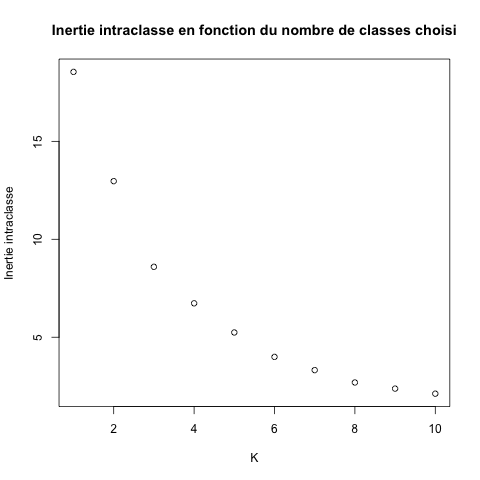
\includegraphics[width=0.5\textwidth]{imgs/K_means_choix_K.png}
        \caption{Inertie intraclasse en fonction du nombre de classes choisi}
        \label{fig_K_means_choix_K}
    \end{figure}

    En utilisant la règle du coude un nombre de classes est 3.
    Ce nombre est en adéquation avec la classification hiérarchique ascendante que nous avions obtenue dans la question précédente.
    En effet nous avions déjà identifié 3 groupes.

    Nous obtenons la classification suivante:
    \begin{center}
        \begin{tabular}{|l|l|l|}
            \hline
            1 & African, Cajun\_Creole, Central\_SouthAmerican, Greek, Indian, Italian, Mediterranean, Mexican, \\
            & MiddleEastern, Moroccan, Southwestern, Spanish\_Portuguese\\
            \hline
            2 & Asian, Chinese, Japanese, Thai, Vietnamese\\
            \hline
            3 & American, EasternEuropean\_Russian, English\_Scottish, French, German, Irish, Jewish,\\
            & Scandinavian, Southern\_SoulFood\\
            \hline
        \end{tabular}
    \end{center}
    Cette classification est identique aux trois groupes que nous avions identifiés précedemment avec la CAH.

    \subsection*{Question 5}

    La classification à 3 groupes ne permet pas d'identifier clairement 3 zones géographique bien distinctes. On se propose alors d'augmenter le nombre de groupes.

    On se propose donc d'identifier 4 groupes. Nous obtenons la classification suivante:
     \begin{center}
        \begin{tabular}{|l|l|l|l|}
            \hline
            1 & Asian, Chinese, Japanese, Thai, Vietnamese\\
            \hline
            2 & Southwestern, Mexican, Indian, Central\_SouthAmerican, Cajun\_Creole\\
            \hline
            3 & Southern\_SoulFood, Scandinavian, Jewish, Irish, German, French, English\_Scottish, \\
            & EasternEuropean\_Russian, American\\
            \hline
	 4 & Spanish\_Portuguese, Moroccan, MiddleEastern, Mediterranean, Italian, Greek, African\\
            \hline
        \end{tabular}
    \end{center}     

    On distingue :
    \begin{itemize}
        \item les pays Sud-Asiatiques
        \item les pays d'Amérique du Sud
        \item les pays du Nords (Europe, Russie, EU)
        \item et les pays du bassin méditéranéen
    \end{itemize}
    Une classification géographique en 4 groupes est comparable à la classification obtenue. Le seul élément qui a été déplacé dans la classification géographique arbitraire est l'Inde.


    \subsection*{Question 6}
    Le jeu de données qui est fourni contient un échantillon avec 2000 recettes (2000 lignes).
    Il y a 26 régions (les mêmes que dans le jeu de données précédent) et 51 variables.
    Les valeurs sont binaires, 0 pour l'absence et 1 pour la présence d'un ingrédient.
    Il n'y a aucune valeur manquante.
    
    \subsection*{Question 7}

    Nous transformons les données en tableau individu-variable: les individus sont les ingrédients et les variables sont les recettes.
   
    Pour calculer la matrice de similarité/dissimilarité nous n'utilisons pas les distances euclidienne et manhattan.
    En effet, si nous prenons deux individus:\\
    0 0 0 0 0 1 0\\
    0 0 1 0 0 0 0\\
    la distance euclidienne est $\sqrt{2}$ ce qui semble faible alors que les deux ingrédients n'ont jamais été utilisés ensemble. 
    La distance euclidienne dépend de la fréquence d'utilisation de deux ingrédients. 
    Deux ingrédients peu utilisés sont proches au sens euclidien car ils sont peu utilisés.
    La distance euclidienne ne mesure pas tellement le degré d'utilisation conjointe.

    Une meilleure mesure de dissimilarité consiste à ne compter seulement les couples (un couple par variable) où il y a au moins un 1.
    
    Nous notons:
    \begin{itemize}
        \item $M_{01}$ le nombre de couples (0,1)
        \item $M_{10}$ le nombre de couples (1,0)
        \item $M_{11}$ le nombre de couples (1,1)
    \end{itemize}

    Une mesure de dissimilarité est:

    \begin{equation}
        \nonumber
        d = \frac{M_{01}+M_{10}}{M_{01}+M_{10}+M_{11}}
    \end{equation}

    Cette mesure est comprise entre 0 et 1. \\
    0 pour deux ingrédients qui sont systématiquement utilisés conjointement.
    1 pour deux ingrédients qui ne sont jamais utilisés conjointement.

    Cette mesure est implémentée dans R avec la fonction "dist" et l'argument method="binary" et est appelée distance de Jaccard. 
    
    \subsection*{Question 8}
    En utilisant la distance de Jaccard et le critère de Ward nous obtenons la classification hiérarchique ascendante suivante:
    \begin{figure}
        \centering
        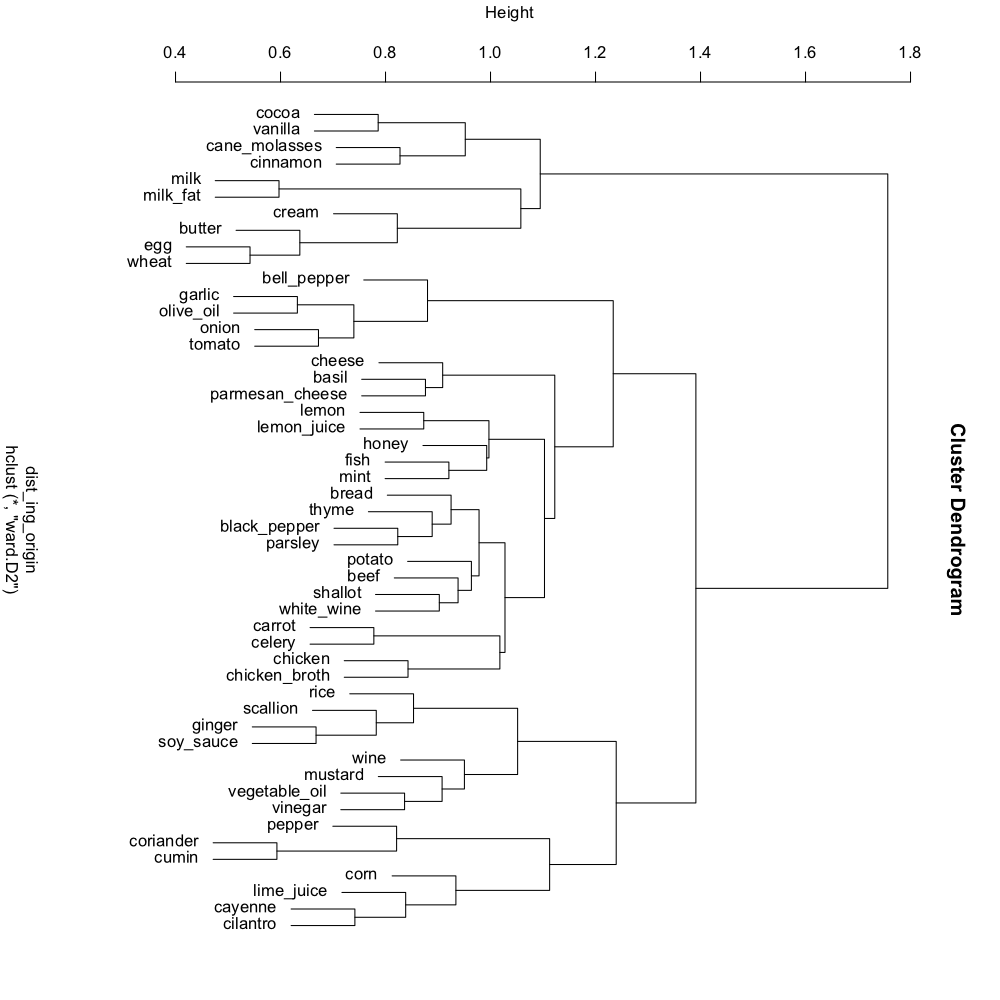
\includegraphics[width=0.8\textwidth]{imgs/CAH_dendrogramme_ingredients_binary.png}
        \caption{Dendrogramme obtenue avec la distance de Jaccard et le critère de Ward}
        \label{fig_K_means_choix_K}
    \end{figure}

    Trois classes d'ingrédients se distinguent:
    \begin{itemize}
        \item les ingrédients pour les desserts
        \item les ingédients pour le plat principal
        \item les ingrédients qui viennent s'ajouter au reste: les condiments, huiles et vin
    \end{itemize}

    \subsection*{Question 9}

    En appliquant l'algorithme des K-médoïdes, avec K=3, au tableau de dissimilarités établi à la question 7 nous obtenons 3 médoides.
    Ces médoïdes nous donnent des ingrédients représentant chaque classe.
    Un ingrédient représentant la première classe est l'oeuf.
    L'onion représente la deuxième classe. Le gingembre représente la dernière classe.

    \section{Classification par K-means avec distance adaptative}
    \subsection{Programmation}

    \subsection{Application}
    Nous testons l'algorithme des K-means à distance adpatative à l'aide de jeux de données synthétiques, puis, comparons les résultats avec l'algorithme des K-means classique (utilisant la distance euclidienne).

    Jeu de données synthétiques 1:


    \begin{figure}
        \centering
        \begin{subfigure}{.5\textwidth}
          \centering
          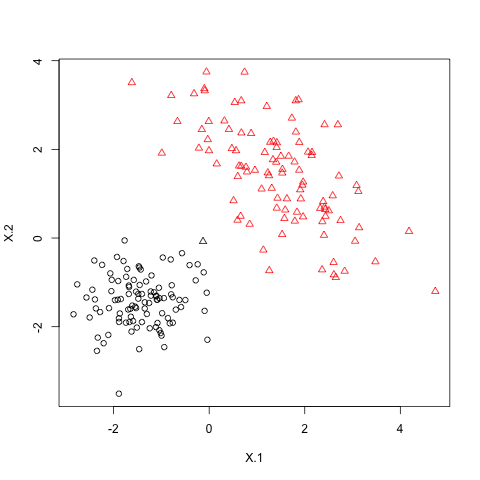
\includegraphics[width=.8\linewidth]{imgs/K_means_synth_1.png}
          \caption{Algorithme des K-means.}
          %\label{fig:sub1}
        \end{subfigure}%
        \begin{subfigure}{.5\textwidth}
          \centering
          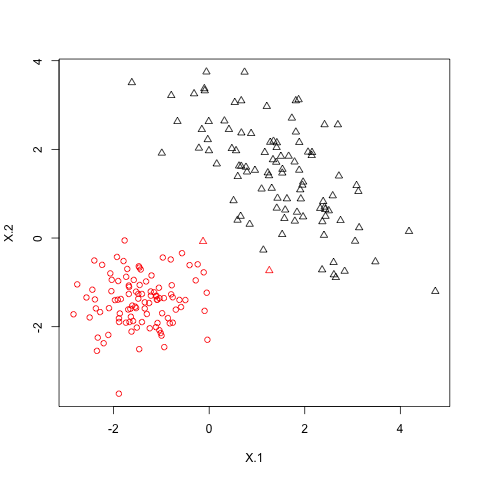
\includegraphics[width=.8\linewidth]{imgs/K_means_adapt_synth_1.png}
          \caption{Algorithme des K-means à distance adaptative.}
          %\label{fig:sub2}
        \end{subfigure}
        \caption{Clusterings effectués sur le jeu de données synthétiques 1. Les couleurs représentent les ensembles trouvés à l'aide des K-means, les symboles des points représentent les vraies partitions.}
        \label{fig_synth_1}
    \end{figure}

    Les deux clusterings obtenus à l'aide des deux méthodes sont très proches.
    Le Rand index ajusté des K-means "classiques" est de 0.98 et Rand index ajusté des K-means à distance adaptative est de 0.96.
    Ces deux scores sont très bons puisque le maximum est de 1. Les partitions trouvées sont donc très proches des vraies partitions.


    Jeu de données synthétiques 2:
    \begin{figure}
        \centering
        \begin{subfigure}{.5\textwidth}
          \centering
          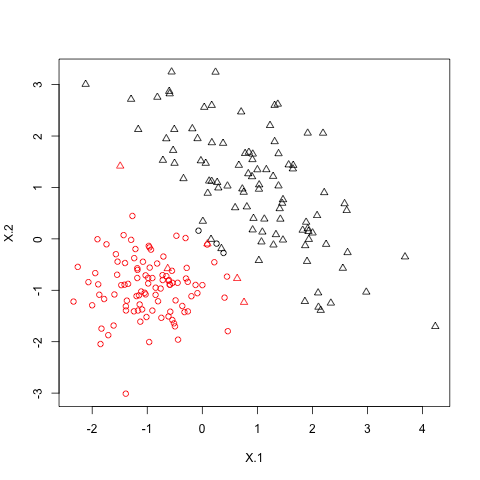
\includegraphics[width=.8\linewidth]{imgs/K_means_synth_2.png}
          \caption{Algorithme des K-means.}
          %\label{fig:sub1}
        \end{subfigure}%
        \begin{subfigure}{.5\textwidth}
          \centering
          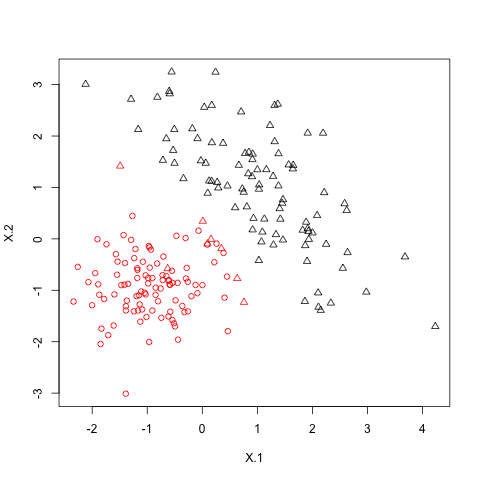
\includegraphics[width=.8\linewidth]{imgs/K_means_adapt_synth_2.png}
          \caption{Algorithme des K-means à distance adaptative.}
          %\label{fig:sub2}
        \end{subfigure}
        \caption{Clusterings effectués sur le jeu de données synthétiques 2. Les couleurs représentent les ensembles trouvés à l'aide des K-means, les symboles des points représentent les vraies partitions.}
        \label{fig_synth_2}
    \end{figure}

    Les deux clusterings obtenus à l'aide des deux méthodes sont très proches.
    Les Rand index ajustés des K-means sont tous les deux de 0.85. Les partitions trouvées sont donc très proches des vraies partitions.
    
    Jeu de données synthétiques 3:
    \begin{figure}
        \centering
        \begin{subfigure}{.5\textwidth}
          \centering
          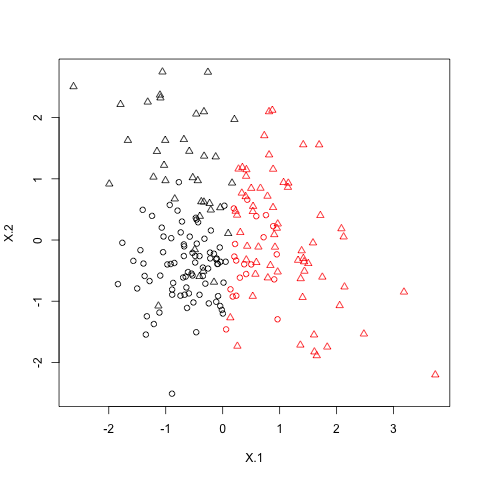
\includegraphics[width=.8\linewidth]{imgs/K_means_synth_3.png}
          \caption{Algorithme des K-means.}
          %\label{fig:sub1}
        \end{subfigure}%
        \begin{subfigure}{.5\textwidth}
          \centering
          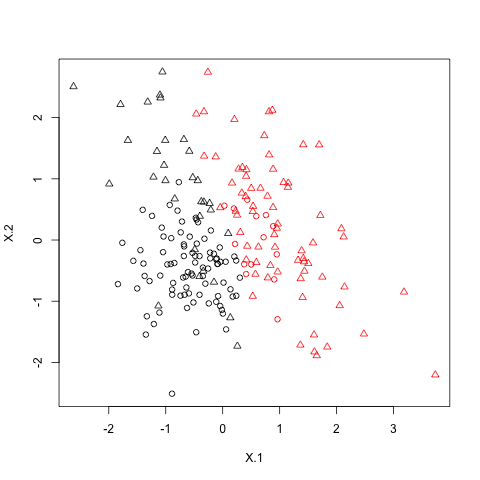
\includegraphics[width=.8\linewidth]{imgs/K_means_adapt_synth_3.png}
          \caption{Algorithme des K-means à distance adaptative.}
          %\label{fig:sub2}
        \end{subfigure}
        \caption{Clusterings effectués sur le jeu de données synthétiques 3. Les couleurs représentent les ensembles trouvés à l'aide des K-means, les symboles des points représentent les vraies partitions.}
        \label{fig_synth_3}
    \end{figure}
    Les deux clusterings obtenus à l'aide des deux méthodes sont cette fois assez différents.
    Les deux ensembles qui forment la vraie partition sont collés tout en ayant une dispersion très différente.
    En effet, l'un a une dispersion faible (inertie par rapport au centre de gravité de 0.17) alors que le second a une dispersion élevée (inertie par rapport au centre de gravité de 0.71).
    L'algorithme des K-means "classiques" ne prend pas en compte la dispersion des classes et sépare donc mal les classes.
    L'algorithme des K-means à distance adaptative prend en compte cette dispersion et sépare donc mieux les données.
    Le Rand index ajusté des K-means "classiques" est de 0.04 et Rand index ajusté des K-means à distance adaptative est de 0.30.
    Les partitions trouvées sont donc assez éloignées des vraies partitions mais l'algorithme des K-means à distance adpatative fait bien mieux que les K-means "classiques".
    
    Iris:

    Nous déterminons les classifications avec les deux méthodes pour K=2,...,5. 
    Nous obtenons les valeurs de criteres, en fonction de K, suivant:
    \begin{figure}
        \centering
        \begin{subfigure}{.5\textwidth}
          \centering
          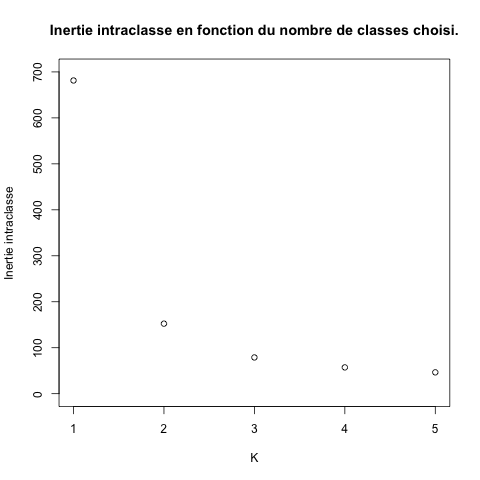
\includegraphics[width=.8\linewidth]{imgs/K_means_Iris_critere.png}
          \caption{Algorithme des K-means.}
          %\label{fig:sub1}
        \end{subfigure}%
        \begin{subfigure}{.5\textwidth}
          \centering
          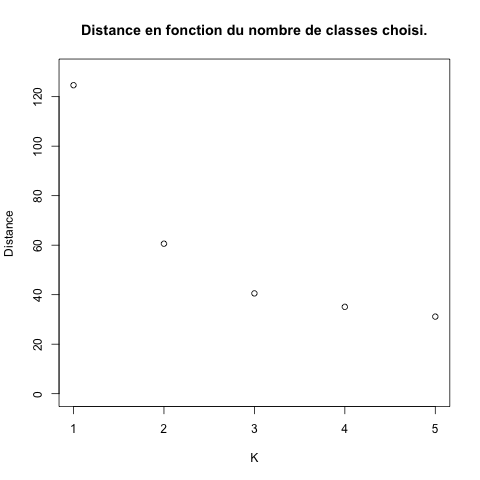
\includegraphics[width=.8\linewidth]{imgs/K_means_adapt_Iris_critere.png}
          \caption{Algorithme des K-means à distance adaptative.}
          %\label{fig:sub2}
        \end{subfigure}
        \caption{Valeurs des critères en fonction de K sur le jeu de données des Iris.}
        \label{fig_Iris_crit}
    \end{figure}

    Pour les K-means un bon K est K=2 (en utilisant la méthode du coude).
    Pour les K-means à distance adaptative un bon K est plutôt 3 (toujours en utilisant la méthode du coude).

    \begin{figure}
        \centering
        \begin{subfigure}{.5\textwidth}
          \centering
          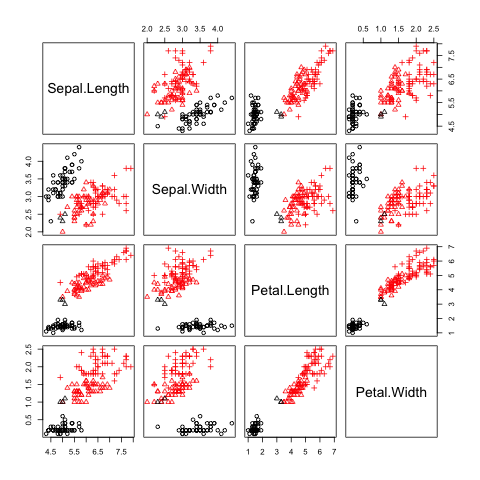
\includegraphics[width=.8\linewidth]{imgs/K_means_iris_2.png}
          \caption{Algorithme des K-means.}
          %\label{fig:sub1}
        \end{subfigure}%
        \begin{subfigure}{.5\textwidth}
          \centering
          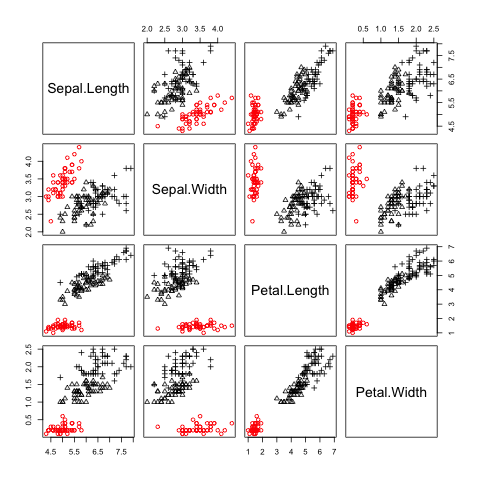
\includegraphics[width=.8\linewidth]{imgs/K_means_adapt_iris_2.png}
          \caption{Algorithme des K-means à distance adaptative.}
          %\label{fig:sub2}
        \end{subfigure}
        \caption{Classification pour K=2 sur le jeu de données des Iris.}
        \label{fig_Iris_2}
    \end{figure}
    
    Pour K=2 nous obtenons deux classifications très similaires.
    En effet deux groupes d'individus se détachent très nettement: un premier avec l'espèce Setosa et un deuxième avec les deux autres espèces.
    La distance adaptative n'apporte donc rien à ce problème de classification pour K=2.
    Les deux index de Rand ajustés sont proches: 0.54 pour les K-means classiques et 0.57 pour les K-means à distance adaptative.
    Les index ne sont pas élevés puisque nous avons mis K=2 alors que le jeu comporte en réalité 3 classes.

    \begin{figure}
        \centering
        \begin{subfigure}{.5\textwidth}
          \centering
          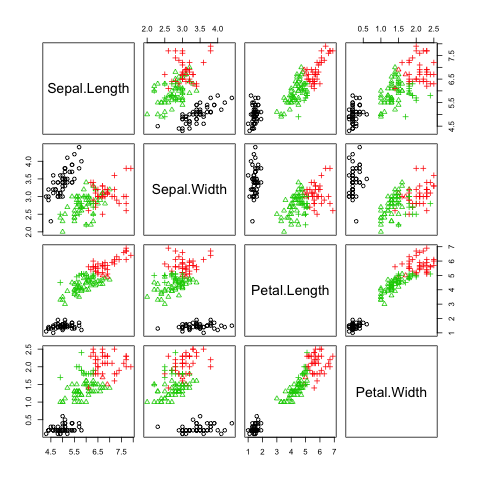
\includegraphics[width=.8\linewidth]{imgs/K_means_iris_3.png}
          \caption{Algorithme des K-means.}
          %\label{fig:sub1}
        \end{subfigure}%
        \begin{subfigure}{.5\textwidth}
          \centering
          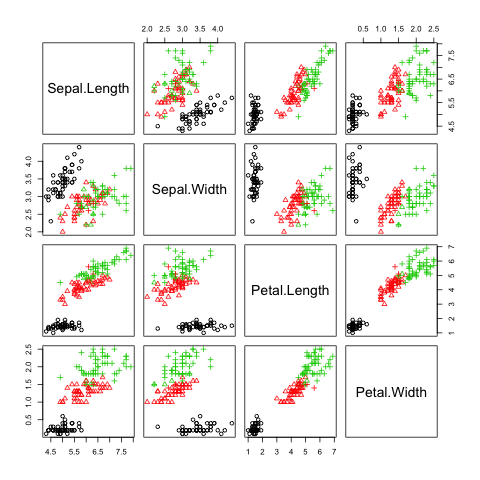
\includegraphics[width=.8\linewidth]{imgs/K_means_adapt_iris_3.png}
          \caption{Algorithme des K-means à distance adaptative.}
          %\label{fig:sub2}
        \end{subfigure}
        \caption{Classification pour K=3 sur le jeu de données des Iris.}
        \label{fig_Iris_3}
    \end{figure}

    Pour K=3, les deux classifications sont assez différentes.
    En effet, dans les deux cas, nous retrouvons un premier groupe avec l'espèce Setosa mais les deux autres groupes sont formés différemment.
    L'algorithme des K-means à distance adaptative sépare les données de manière très proche par rapport aux classes exactes.
    En effet nous avons un index de Rand ajusté de 0.87 alors que pour l'algorithme des k-means classique l'index de Rand est de 0.73.
    Cela s'explique par le fait les K-means à distance adaptative s'adaptent beaucoup mieux aux différentes dispersions des données.
    Les individus de l'espèce Virginica sont bien plus dispersés que ceux de l'espèce Versicolor. Cela est visible sur la figure \ref{fig_Iris_3_sepal_petal}.

    \begin{figure}
        \centering
        \begin{subfigure}{.5\textwidth}
          \centering
          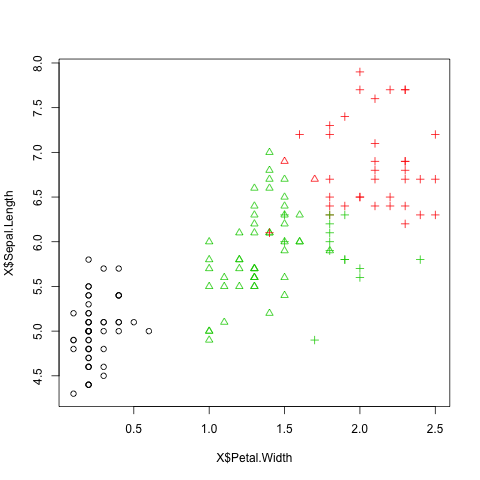
\includegraphics[width=.8\linewidth]{imgs/K_means_iris_3_sepal_petal.png}
          \caption{Algorithme des K-means.}
          %\label{fig:sub1}
        \end{subfigure}%
        \begin{subfigure}{.5\textwidth}
          \centering
          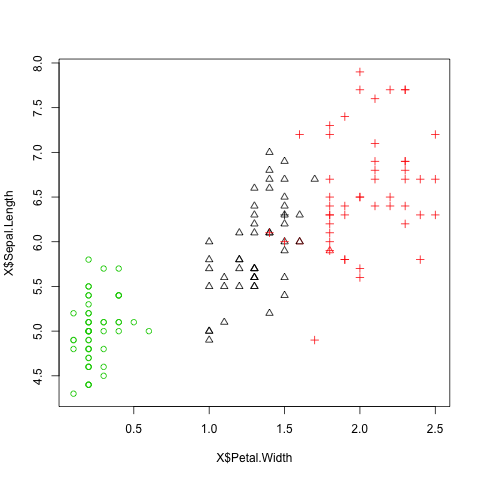
\includegraphics[width=.8\linewidth]{imgs/K_means_adapt_iris_3_sepal_petal.png}
          \caption{Algorithme des K-means à distance adaptative.}
          %\label{fig:sub2}
        \end{subfigure}
        \caption{Classification pour K=3 sur le jeu de données des Iris.(rond: Setosa, triangle: Versicolor, plus: Virginica).}
        \label{fig_Iris_3_sepal_petal}
    \end{figure}

    Spam:

    Nous commençons par traiter les données en utilisant une ACP.
    99.8\% de la variance totale est contenue dans les 2 premiers axes de l'ACP.
    Nous réduisons donc l'espace en un espace de dimension 2.
    \begin{figure}
        \centering
        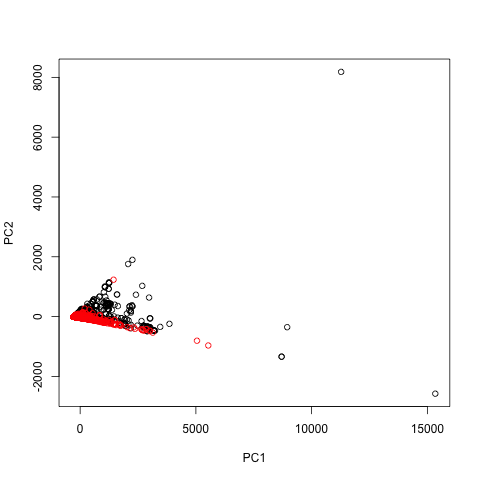
\includegraphics[width=.5\linewidth]{imgs/Spam_ACP.png}
        \caption{Ensemble des données après ACP. Les couleurs représentent les 2 classes.}
        \label{fig_spam_ACP}
    \end{figure}

    Nous pouvons observer sur la figure \ref{fig_spam_ACP} que les spams et non-spams se superposent pour les valeurs négatives du deuxième axe.
    Cette superposition montre qu'il est difficile de trouver une séparation entre les spams et non-spams avec un algorithme non supervisé puisque les algorithmes non supervisés fonctionnent par recherche de similarité.

    En utilisant les K-means à distance adaptative implémenté précédemment nous trouvons la classification visible sur la figure \ref{fig_spam_k_means_adaptative}.
    Malheureusement, le résultat n'est pas très bon puisque l'index de Rand ajusté est de 0.05.
    \begin{figure}
        \centering
        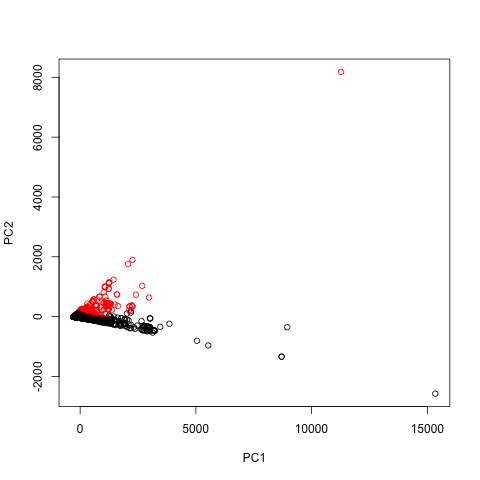
\includegraphics[width=.5\linewidth]{imgs/Spam_ACP_k_means_adaptative.png}
        \caption{Classification en utilisant les k-means à distance adaptative. Les couleurs représentent les 2 classes.}
        \label{fig_spam_k_means_adaptative}
    \end{figure}

    \subsection{Justification}
    \subsection*{Question 10}
    \begin{equation}
        J(\{v_k, M_k\}_{k=1,...,K}) = \sum^{K}_{k=1}\sum^{n}_{i=1} z_{ik} \big[ (x_i-v_k)^\top M_k (x_i-v_k)\big]
    \end{equation}

    Soit $k\in \{1,...,K\}$

    \begin{equation}
        \frac{\partial J(\{v_k, M_k\})}{\partial v_k} = -\sum^{n}_{i=1} z_{ik} (M_k + {M_k}^\top) (x_i-v_k) = -(M_k + {M_k}^\top) \sum^{n}_{i=1} z_{ik} (x_i-v_k)
    \end{equation}

    Nous cherchons quand 

    \begin{equation}
        \frac{\partial J(\{v_k, M_k\})}{\partial v_k} = 0
    \end{equation}

    Comme $M_k$ est quelconque, il faut que:

    \begin{equation}
        \sum^{n}_{i=1} z_{ik} (x_i-v_k) = 0
    \end{equation}
    
    En supposant $n_k \neq 0$:

    \begin{equation}
        \implies n_k \overline{x_k} - \sum_{i\in P_k} v_k = 0 \ avec \ \overline{x_k} = \frac{1}{n_k}\sum_{i=1}^{n}z_{ik}x_i
    \end{equation}

    \begin{equation}
        \implies n_k \overline{x_k} - n_k v_k = 0
    \end{equation}
    
    \begin{equation}
        \implies v_k = \overline{x_k} = \frac{1}{n_k}\sum_{i=1}^{n}z_{ik}x_i
    \end{equation}

    \subsection*{Question 11}

    \begin{equation}
        J(\{v_k, M_k\}_{k=1,...,K}) = \sum^{K}_{k=1}\sum^{n}_{i=1} z_{ik} \big[ (x_i-v_k)^\top M_k (x_i-v_k)\big]
    \end{equation}

    Soit $k\in \{1,...,K\}$

    \begin{equation}
        \frac{\partial L(\{v_k, M_k, \lambda_k\})}{\partial M_k} = \frac{\partial J(\{v_k, M_k\})}{\partial M_k} - \frac{\partial\big[ \sum^{K}_{q=1} \lambda_q (det M_q - \rho_q)\big]}{\partial M_k}
    \end{equation}

    \begin{equation}
        \frac{\partial J(\{v_k, M_k\})}{\partial M_k} = \sum^{n}_{i=1} z_{ik} \frac{\partial \big[(x_i-v_k)^\top M_k (x_i-v_k)\big]}{M_k} =  \sum^{n}_{i=1} z_{ik} (x_i-v_k)(x_i-v_k)^\top
    \end{equation}
    
    \begin{equation}
        \frac{\partial \big[\sum^{K}_{q=1} \lambda_q (det M_q - \rho_q)\big]}{\partial M_k} = \lambda_k \frac{\partial det M_k}{\partial M_k} = \lambda_k det M_k ({M_k}^{-1})^\top
    \end{equation}

    donc,
    \begin{equation}
        \frac{\partial L(\{v_k, M_k, \lambda_k\})}{\partial M_k} = \sum^{n}_{i=1} z_{ik} (x_i-v_k)(x_i-v_k)^\top - \lambda_k det M_k ({M_k}^{-1})^\top
    \end{equation}

    Nous cherchons quand 

    \begin{equation}
        \frac{\partial L(\{v_k, M_k, \lambda_k\})}{\partial M_k} = 0
    \end{equation}

    donc,

    \begin{equation}
        \lambda_k det M_k ({M_k}^{-1})^\top = \sum^{n}_{i=1} z_{ik} (x_i-v_k)(x_i-v_k)^\top
    \end{equation}

    en supposant que $det M_k \neq 0$ et $\lambda_k \neq 0$

    \begin{equation}
        \iff ({M_k}^{-1})^\top = \frac{1}{\lambda_k det M_k }\sum^{n}_{i=1} z_{ik} (x_i-v_k)(x_i-v_k)^\top
        \label{eq_8}
    \end{equation}

    en appliquant la transposée de chaque côté de l'équation et $(A+B)^\top = A^\top + B^\top$ et $(AB)^\top = B^\top A^\top$

    \begin{equation}
        \iff {M_k}^{-1} = \frac{1}{\lambda_k det M_k }\sum^{n}_{i=1} z_{ik} (x_i-v_k)(x_i-v_k)^\top
    \end{equation}

    \begin{equation}
        \iff {M_k}^{-1} = \frac{n_k}{\lambda_k det M_k }V_k \ avec \ V_k = \frac{1}{n_k}\sum^{n}_{i=1} z_{ik} (x_i-v_k)(x_i-v_k)^\top
        \label{eq_9}
    \end{equation}

    De plus, comme $J$ ne dépend pas de $\lambda_k$:

    \begin{equation}
        \frac{\partial L(\{v_k, M_k, \lambda_k\})}{\partial \lambda_k} = detM_k - \rho_k
    \end{equation}
    
    Nous cherchons quand,

    \begin{equation}
        \frac{\partial L(\{v_k, M_k, \lambda_k\})}{\partial \lambda_k} = 0
    \end{equation}
    \begin{equation}
        \iff detM_k = \rho_k
        \label{eq_13}
    \end{equation}
    Donc si $\rho_k \neq 0$ alors $det M_k \neq 0$, ce qui montre que l'hypothèse faite pour obtenir l'équation \ref{eq_8} est réaliste.

    En combinant les équations \ref{eq_9} et \ref{eq_13}, nous obtenons:

    \begin{equation}
        {M_k}^{-1} = \frac{n_k}{\lambda_k \rho_k }V_k \ avec \ V_k = \frac{1}{n_k}\sum^{n}_{i=1} z_{ik} (x_i-v_k)(x_i-v_k)^\top
        \label{eq_14}
    \end{equation}

    Donc, (en supposant $n_k \neq 0$):
    \begin{equation}
        \implies V_k = \frac{\lambda_k \rho_k}{n_k} {M_k}^{-1}
    \end{equation}

    \begin{equation}
        \implies det(V_k) = det(\frac{\lambda_k \rho_k}{n_k} {M_k}^{-1})
    \end{equation}

    En utilisant la multilinéarité du déterminant et le fait que $V_k$ soit une matrice carrée de taille $p$:
    \begin{equation}
        \implies det(V_k) = \frac{{\lambda_k}^p {\rho_k}^p}{{n_k}^p} det({M_k}^{-1})
    \end{equation}

    De plus $det({M_k}^{-1}) = \frac{1}{det(M_k)} = \frac{1}{\rho_k}$

    \begin{equation}
        \implies \rho_k det(V_k) = \frac{{\lambda_k}^p {\rho_k}^{p}}{{n_k}^p}
    \end{equation}

    \begin{equation}
        \implies \frac{{n_k}^p}{{\lambda_k}^p} = \frac{{\rho_k}^{p}}{\rho_k det(V_k)} 
    \end{equation}

    \begin{equation}
        \implies \frac{n_k}{\lambda_k \rho_k} = \frac{1}{{\rho_k}^{\frac{1}{p}}{det(V_k)}^{\frac{1}{p}}}
        \label{eq_20}
    \end{equation}

    En combinant les équations \ref{eq_14} et \ref{eq_20} nous obtenons:

    \begin{equation}
        {M_k}^{-1} = \frac{1}{{\rho_k}^{\frac{1}{p}}{det(V_k)}^{\frac{1}{p}}}V_k \ avec \ V_k = \frac{1}{n_k}\sum^{n}_{i=1} z_{ik} (x_i-v_k)(x_i-v_k)^\top
    \end{equation}

    \begin{equation}
        \implies {M_k}^{-1} = (\rho_k det(V_k))^{-\frac{1}{p}}V_k \ avec \ V_k = \frac{1}{n_k}\sum^{n}_{i=1} z_{ik} (x_i-v_k)(x_i-v_k)^\top
    \end{equation}

    \end{document}

